\chapter{Software Re-engineering}

\label{Chapter3}

This section covers a simplified process of software re-engineering.
Rhat is a process for taking an existing system developing an understanding of how it works, then refactoring that system and engineering changes, then implementing the system as to the conclusions made during refactoring.

Reverse engineering is the process of reviewing the existing software systems and documenting how they function. This can be done through diagramming, documenting, and refactoring. This process allows the engineer to understand the problem domain of the system more, and also provides information on parts of the software that need to be restructured and changed.

Restructuring is the process of taking an existing design and making changes to improve the design. This is the main transitional phase that will happen after the original understanding of how the current system works through reverse engineering. Restructuring will involve reorganizing code as granular or abstract as desired. Most restructuring will focus on making small changes to the system to make it more maintainable or run more efficiently. However, the restructuring of the current system will appear to be more of an overhaul.

% Need to expand this section.
Forward engineering is the process of taking the results of the system specification created from the two previous steps of the reengineering process integrating the system into the code-base.

\section{System Understanding}

The system is arranged for the most part into different functional groups, referred to as packages. There are some exceptions to this as seen in the "ai" package, where the responsibility of controls, vision, and movement is all amalgamated together.

The flow of information is handled quite elegantly within the system.
With lower level systems passing information up to and receiving back from
higher level systems. See \ref{fig:InformationFlow} for understanding the
general idea of how this flow happens.

\begin{figure}
\centering
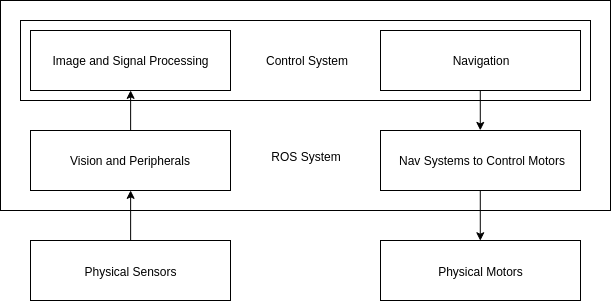
\includegraphics[width=100mm]{Figures/InformationFlow}
\decoRule
\caption[Original Information Flow]{Diagram showing how information flows in the reference frame of the control system.}
\label{fig:InformationFlow}
\end{figure}

The individual devices are handled via their own ROS nodes, which then make
the information from the devices available in a 'friendly' way.
This allows for specific driver-like programs to abstract the possibly
complex interface to the physical devices.


\section{Perceived Problems}

The control system featured no error catching or any kind of protocol to recover from an error state.
For most states the control system loops on a single state then after a condition is met will advance to the next state. This type of control system is autonomous controlling but it isn't designed for the kind of failures expected in the real world.

The control system works directly with the state information and directly handles both the condition to switch states and the assignment of the next state, see \ref{fig:DirectStateHandling}.

\begin{figure}
\centering
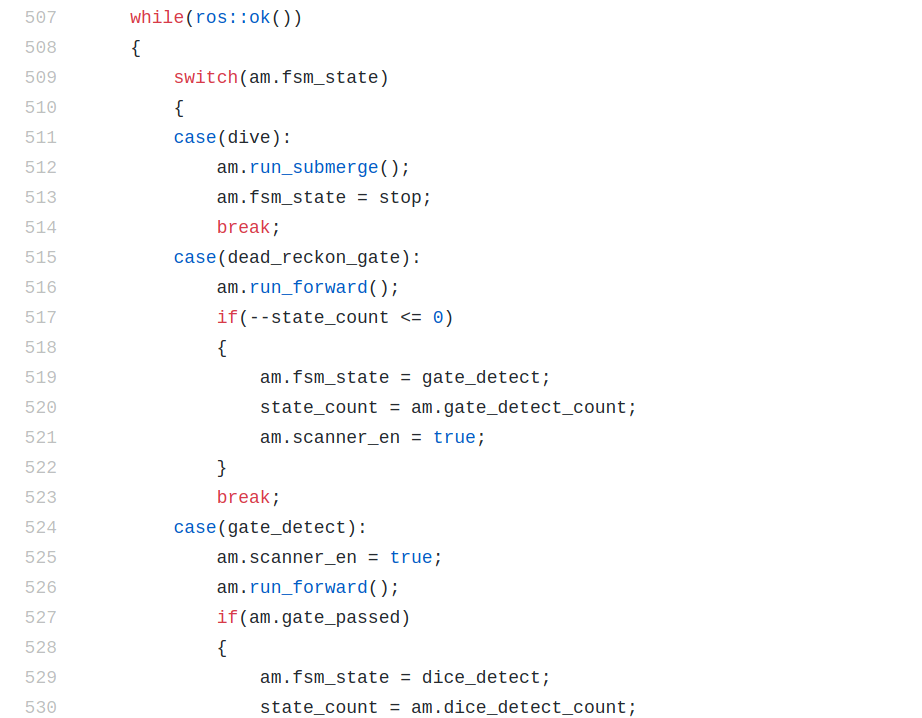
\includegraphics[width=150mm]{Figures/DirectStateHandling}
\decoRule
\caption[Direct State Handling]{Code segment showing the control systems way of handling states, controlling submarine functions, and getting information from other submarine systems.}
\label{fig:DirectStateHandling}
\end{figure}

The control system also directly handled the vision systems. The control system did offer a simple interface for the states in the state machine to utilize.


\section{Restructuring}

\subsection{Overview}
The control system has been assigned excessive responsibility; it performs the
tasks of a control system, detection system, and navigation system.
The detection systems within the control system shall be separated into a vision
package and offer an interface through ROS inter process communication
structures.
Namely offer the same features the state machine was using, and expand the
features on top of that.
And the navigation system uses should also be pulled out, but an interface still
be made available through ROS inter-process communication structures.
To use the two new systems identified above they would need to be compatible
with the existing system structure.

For the navigation system this required either using interface that existed and
offered functionalities by replaced system, or a new system that acts as an
interface to manage communication between old and new software systems.
The latter involved much more consideration for best creating the system for
usage in the future.
While the former got the job done, and allowed to expand and slowly update
functionality later on.
Thus, the former of the two options was chosen, for the reasons given and
because of time constraints for the project.

The detection systems' functionality and usage was restricted to within the
control system.
This allowed creation of a new system much simpler and allowed much freedom with
the design of this system.
Which is why the system used a simple interface to retrieve detection results,
and change detection type.
And this system was incorporated directly into the vision package, as having
close proximity to the retrieved image files would mean for faster image
processing.
However, this document's purpose is the redesign of the control system and this
won't cover the new design of the detection system.

The updated version of the ROS communication diagram was too large to embed into
this document, but it has been provided \href{https://drive.google.com/file/d/1_vJLSflxahA-7v2kYGV3wu5SfGcKEVf8/view?usp=sharing}{here}.

\begin{figure}[H]
\centering
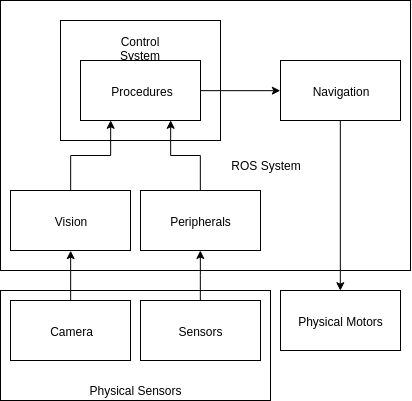
\includegraphics[width=100mm]{Figures/InformationFlowNew}
\decoRule
\caption[New Information Flow]{Diagram showing how information flows in the reference frame of the redesigned control system.}
\label{fig:InformationFlowNew}
\end{figure}

\begin{figure}[H]
\centering
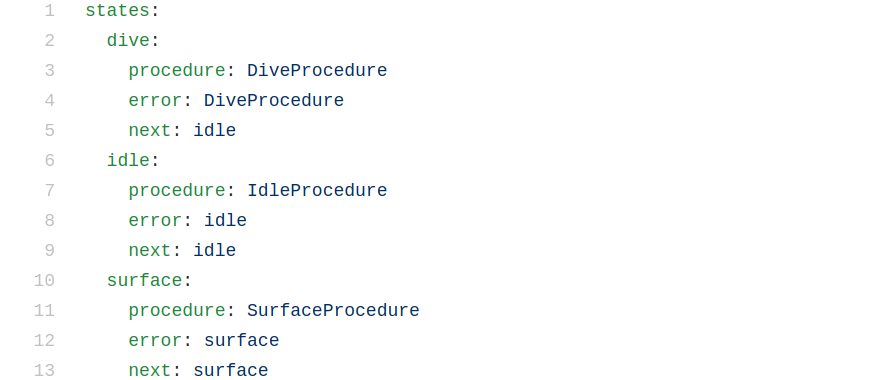
\includegraphics[width=150mm]{Figures/ExampleConfig}
\decoRule
\caption[Example Configuration File]{Shows a simple example idle configuration file. Demonstrating use of simple state organization and definition of state transitions.}
\label{fig:ExampleConfig}
\end{figure}

\subsection{Control System Specification}

This section will focus on the specific design of the new control system that is
intended to replace the existing control system.
Specifics will be provided for the format of the dynamic state configuration
file, as well as the procedures that will be defined to use with the new state machine.

\subsubsection{State Machine - Configuration Specification}

State configurations are define in a YAML file and are loaded as an argument
through the launch file for the control system package.
The configuration file must have a root tag 'states' which is a dictionary of
either all state or state lists.
To differentiate between a state and a state list restrictions must be placed on
what must be in a state, and what must not be in a state list.
It is also to note that the root dictionary, labeled states, would be classified as a
state list.

State lists are dictionaries containing keys being the state names, and values
being the state parameters.
State lists must not use reserved words, listed below in
\ref{tab:StateRequiredFields}, or required state names, listed below in
\ref{tab:RequiredStateNames} their names.

States are dictionaries containing the fields listed in
\ref{tab:StateRequiredFields}. State names cannot be the same as the name of the
fields that the states themselves have as part of their dictionaries, as this
would severely complicate the parser.

\begin{table}[]
  \begin{tabular}{|l|l|}
    \hline
    Field & Description \\ \hline
    procedure & This defines the c++ procedure that this state relies on. \\ \hline
    error     & This specifies the path name of the state this state transitions to for error behaviour. \\ \hline
    next      & This specifies the path name of the state this state transitions to for normal behaviour. \\ \hline
  \end{tabular}
  \caption[State Reserved Words and Descriptions]{List of reserved words for states and their meaning.}
  \label{tab:StateRequiredFields}
\end{table}

\begin{table}[]
  \begin{tabular}{|l|l|}
    \hline
    State Name & Description \\ \hline
    dive & This state represents the start state for the state machine. \\ \hline
    surface & This state represents the end state for the state machine. \\ \hline
  \end{tabular}
  \caption[Required States and Descriptions]{List of required states and their expected function.}
  \label{tab:RequiredStateNames}
\end{table}

\subsubsection{State Machine - Procedures}

Each procedure will be derived from the base procedure class.
This allows the use of virtual functions to ensure that each derived procedure
class is implementing the appropriate methods and also to simplify creation of
procedure objects when loading states dynamically.

\lstset{language=C++}
\begin{lstlisting}
  class Procedure {
    public:
    // Enum class used to literately inform control
    // system of meaning of return code.
    // (e.g., accessed via Procedure::ReturnCode::NEXT)
    enum class ReturnCode : int {
      FATAL,
      ERROR,
      CONTINUE,
      NEXT
    };

    // Left default, but derived procedures are free to have
    // various members and initialize them however they please.
    Procedure() = default;


    // This is the function for carrying out the
    // procedure functionality will return a result
    // which informs the state machine when it's
    // ready to advance to the next state, continue with
    // the current state, or if it's encountered an error.
    virtual ReturnCode operator()() = 0;
  }
\end{lstlisting}

\section{Forward Engineering}

\subsection{Preparing Procedures}

The state machine needs to have a list of all the available procedures that it
has to work with before it can begin to parse the states from the configuration
file.
This is done by first creating a map with the key being a string with the same
name as the procedure object, and a value being an instance of the function
object.
This allows for the parser to look up the procedure from the provided name, and
throw an error if a procedure cannot be found.
When the procedures are loaded from the parsing new instances of the function
object are created, which allows for state of the function object to be unique
to the state of control system it is being loaded with.
It is also worth noting that if behaviour was desired where each state in the
control system had state information from a procedure of the same type being
used elsewhere in the system that could be accomplished by using static object
members.

\subsection{Dynamic State Loading}
Implementing the configuration parser that would be used to parse the
configuration provided was made a lot easier through ROS' parameter server
library.
Using it the configuration files are automatically broken up into a logical
representation of what was in the configuration file.
The parser starts with the root tag of the configuration file which it parses as a
state list, then identifies all the items within as either a state or a list of
more states.
If it's a state it will generate a logical representation of that state,
otherwise it will add it to the list of things to parse like it did with the
root state list.
The only required work was to structure code to look for identifiers for when
the parser had encountered a state or if it needed to add more suspect states to
the 